\documentclass[11pt]{article}
\usepackage[utf8]{inputenc}
\usepackage{graphicx}
\usepackage{titlepic}
\usepackage{caption}
\usepackage{subcaption}
\usepackage[a4paper, total={6in, 8in}]{geometry}

% \documentclass{beamer}
\usepackage{amsmath}

\newcommand{\namesigdate}[2][5cm]{%
  \begin{tabular}{@{}p{#1}@{}}
    #2 \\[0.4\normalbaselineskip] \hrule \\[0pt]
    {\small } \\[2\normalbaselineskip] 
  \end{tabular}
}

\title{\vspace*{\fill} \textbf{Audio Description and Content Moderation App}
	  \\ {\large \textbf{Summer Undergraduate Research Award}}
	  \\  \vspace{3mm} 
\includegraphics[width=5cm]{logo.jpg}}

\author{
	\textbf{Ayush Patel}\\ 
	2016CS10396\\
	Computer Science\\
	CGPA: 9.305 \\
	Mob: 9891052662\\
	cs1160396@iitd.ac.in
	\and
	\textbf{Mohit Gupta}\\ 
	2016CS50433\\
	Computer Science\\
	CGPA: 9.579\\
	Mob: 9466479674\\
	cs5160433@iitd.ac.in
}
\date{\textbf{Supervisor:-} \\ \textbf{Aaditeshwar Seth} \\ Professor \\ Department of CSE \\ aseth@cse.iitd.ac.in\\ IIT Delhi\\
\vspace*{\fill}}




\begin{document}
	\maketitle

\begin{center}
\noindent\rule{3.2cm}{0.4pt} 
\end{center}

\begin{flushright}
\noindent\rule{3.2cm}{0.4pt} 
\\ \textbf{Prof. S. Arun Kumar}
\\ Head of Department
\\ Department of CSE
\\ sak@cse.iitd.ernet.in
\end{flushright}


	\newpage

	\section{Introduction}



	\section{Objectives}


\section{Approach to the project}
		The basic approach is to train our model using audios that already have been segregated into different categories, so that our networks ``learns'' to segregate audios.\\
		In order to achieve this we have broken down our problem in several parts. First we will be giving tags to the audios depending on their quality and will try to enhance the quality of poor quality audio. We will reject the audios for which no enhancement is possible. Then the audio is converted to text using Natural language processing (NLP). Using the textual information, we provide hash-tags to the audio and then using a multiclass neural network we assign the probability of the audio falling under a particular topic and  then assigning it the main topic. Then depending on the topic, we decide the abusive tolerance level and then mark the audios with abusive level more than the tolerance level for consideration from moderator. Depending on the scores of the moderator, if the combined score of the moderators who mark the audio as ``Rejected`` is above a certain level, then the audio is moved to trash. The scores to the moderators (and community reporters) is given using a standard scoring algorithm which will be developed in future. Then after passing through all the stages, the audio is available to the user through the app.
		\begin{enumerate}
			\item Audio Quality
			\begin{enumerate}
				\item
					Set up a deep neural network with pre-trained weights to separate noise from the audio.
				\item
					Depending on the output audio file, if the audio is not clear than the audio file is rejected.
			\end{enumerate}
			\item Audio Enhancement
			\begin{enumerate}
				\item
					We will use digital sampling to reconstruct the audio as much as possible.
				\item
					We sample at least twice as fast as the highest frequency we want to record so that we can use Nyquist theorem perfectly reconstruct the original sound wave from the spaced-out samples.				
			\end{enumerate}
			\item Speech Recognition and abuse filtering
			\begin{enumerate}
				\item
					The user is asked to choose one of the provided languages so that it helps us to use a pre-trained neural network to convert audio to text.
                \item
					We will be using APIs like Watson speech to text or Google speech aip for converting the audio to text.
				\item
					Depending on the abusive words in the language, we segregate the audios into abusive tolerable or abusive intolerable.
			\end{enumerate}
			\item Topic Assignment
			\begin{enumerate}
				\item
					We use "one vs all" multi-class classifier neural network for the purpose of hash-tag assignment and topic assignment to the audio.
                \item
					The moderators (or community reporters) may change the topic is the want to do so.
			\end{enumerate}
			\item Further Possibilities
			\begin{enumerate}
				\item
				    We will be training on more languages to accommodate linguistic diversity prominently in rural areas
				\item
				    Apart from the app for content moderators, we may also build an app for users so that they can get news on demand as per their preferences.
			\end{enumerate}
		\end{enumerate}


	\section{Budget and duration}	
		\subsection{Budget}
			No budget is required for this project.			
					
		\subsection{Duration}
			We will try to complete this project by the end of the summer break i.e. the end of July, 2017. 

	\section{Background} 
			\subsection{Deep Learning}
				Deep Learning is a branch of machine learning in which multiple parameter based models are used in series. In a deep network, there are many layers between the input and output, allowing the algorithm to be executed in multiple processing steps, composed of \textbf{multiple linear and non-linear transformations}. At each layer, the signal is transformed by a processing unit, like an artificial neuron, whose parameters are \textbf{`learned'} through training. Deep Learning has been shown to excel in tasks where the goal is to find \textbf{intuitive} patterns in the data.\cite{deep} In particular, in the field of Computer Vision, deep networks are increasingly used to extract \textbf{feature descriptions and inter-relationships between features} from images.\cite{cs231n}
				\begin{figure}[ht!]
					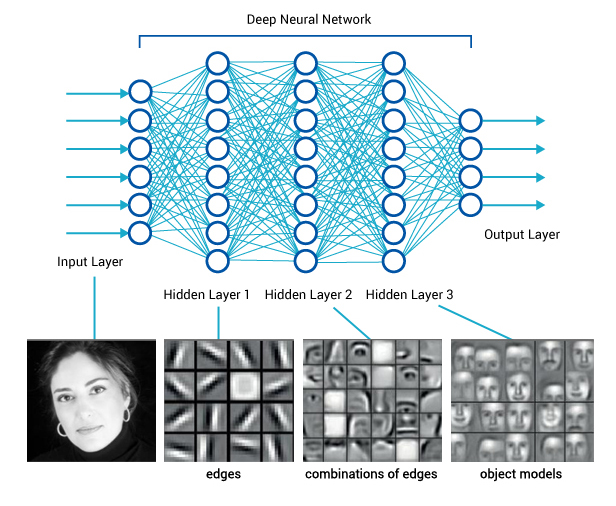
\includegraphics[width=14cm]{blog_deeplearning3.jpg}
					\caption{Illustration of Deep Learning as applied to Vision\label{fig2}}
				\end{figure}	

			\subsection{Convolutional Neural Networks}
			Convolutional Neural Networks (CNN, or ConvNet) are a type of feed-forward artificial neural network in which the connectivity pattern between the neurons is inspired by the organization of the animal visual cortex. Individual cortical neurons respond to stimuli in a restricted region of space known as the \textbf{receptive field}. The receptive fields of different neurons partially overlap such that they tile the visual field. The response of an individual neuron to stimuli within its receptive field can be approximated mathematically by a \textbf{convolution operation}. A Convolutional Neural Network consists of the following layers.\cite{showandtell}
								
				\begin{figure}[ht!]
					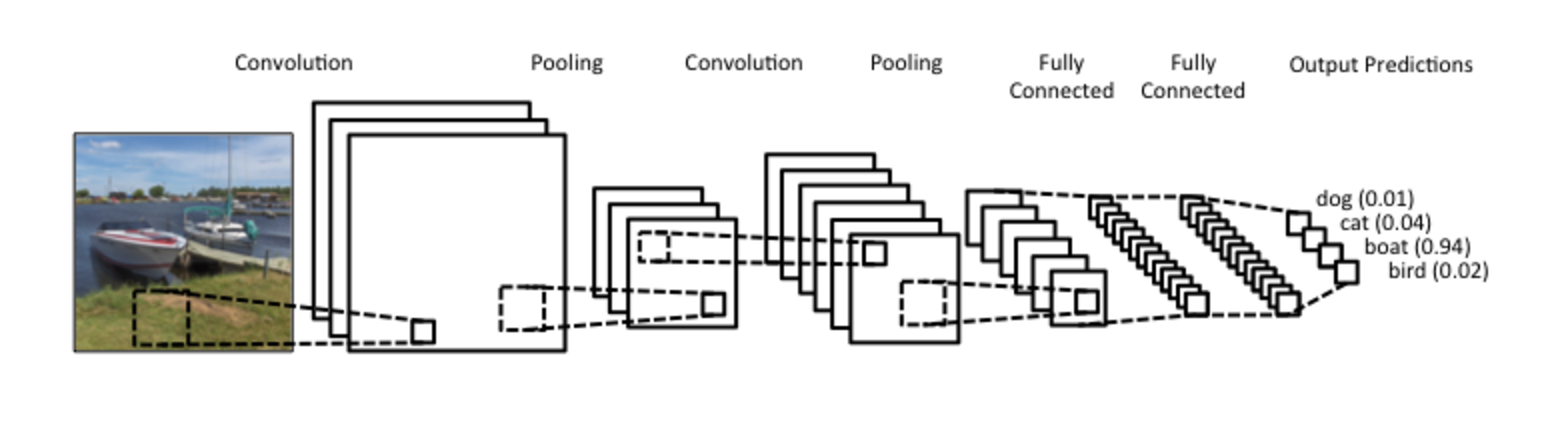
\includegraphics[width=1.0\textwidth]{conv.png}
					\caption{A Typical Convolutional Neural Network\label{fig4}}
				\end{figure}
			%skipping Relu layer since its not in picture assume it to be in conv layer
				\subsubsection{Convolutional Layer}
					The convolution layer is the core building block of a CNN. The layer's parameters consist of a set of \textbf{learnable filters} (or kernels), which have a small receptive field, but extend through the full depth of the input volume. During the forward pass, each filter is convolved across the width and height of the input volume, computing the dot product between the entries of the filter and the input and producing a $2$-dimensional activation map of that filter.\cite{cs231n} As a result, the network learns filters that activate when it detects some specific type of feature at some spatial position in the input.

				% \subsubsection{Max Pooling Layer}
				% 	It is common to periodically insert a Pooling layer in-between successive Conv layers in a ConvNet architecture. Its function is to \textbf{progressively reduce the spatial size} of the representation to reduce the amount of parameters and computation in the network, and hence to also control over-fitting. The Pooling Layer operates independently on every depth slice of the input and resizes it spatially, using the max operation.\cite{cs231n}
				% \subsubsection{Fully-Connected Layer}
				% 	Finally, after several convolutional and max pooling layers, the high-level reasoning in the neural network is done via fully connected layers. Neurons in a fully connected layer have \textbf{full connections to all activations} in the previous layer, as seen in regular Neural Networks. Their activations can hence be computed with a matrix multiplication followed by a bias offset.\cite{fullyconnected} Thus output of the fully connected layer is a vector with elements representing the `probability' (not in a strictly statistical sense) of the image containing specific objects or actions.

% 			\subsection{Long Short Term Memory Networks}
% 			    \begin{figure}[ht!]
% 			    	\centering
% 					\includegraphics[scale=0.266]{LSTM_unit.png}
% 					\caption{A single LSTM unit\label{fig6}}
% 				\end{figure}
% 				Long Short Term Memory Networks are a type of Recurrent Neural Networks. These networks are based upon recursion, so that variable length inputs can be handled easily and sequential information can be processed with better results. LSTM's are specifically used for making RNNs learn long term patterns since traditional RNNs tend to \textbf{favour short term temporal dynamics}. It can be difficult to train traditional RNNs to learn long-term dynamics, likely due in part to the \textbf{vanishing and exploding gradients problem} that can result from propagating the gradients down through the many layers of the recurrent network, each corresponding to a particular time step\cite{ltms}. LSTMs provide a solution by incorporating memory units that explicitly allow the network to learn when to ``forget'' previous hidden states and when to update hidden states given new information\cite{lstmexecute}.\\

		
			\subsection{Training Deep Neural Networks}
					\begin{figure}[ht!]
					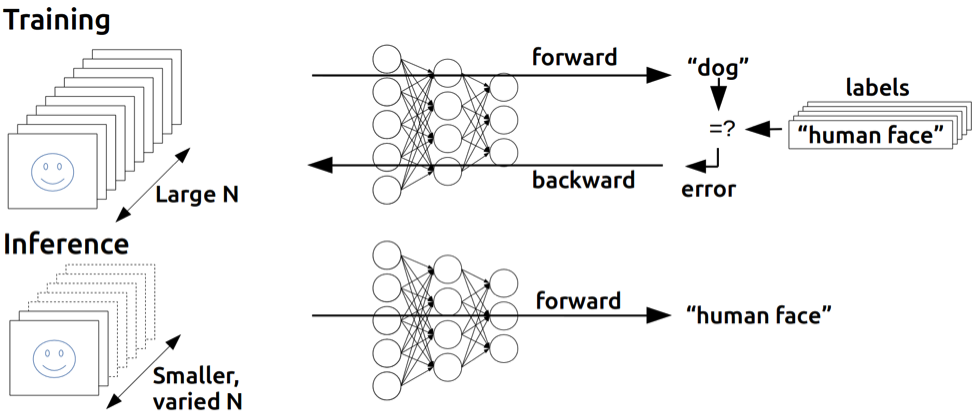
\includegraphics[width=14cm]{training_inference1.png}
					\caption{Training and Inference Processes\label{fig5}}
				\end{figure}
				A Deep Neural Network is at it's core a parameter based function. All of these parameters are  \textbf{trained} automatically from inputs and expected output tuples (training data). The training process revolves around minimizing a particular cost function using methods like \textbf{Stochastic gradient descent}. The input is given to the network in a feed forward fashion and the parameters are modified from the last layer to the first \textbf{(Backpropagation)}. Neural Networks, by design, require huge amounts of training data and take a large time to get trained. For some perspective, most current state of the art image classifiers have $> 100$ million parameters and are trained on more than 1.2 million images. 


% 			\subsection{Finetuning}
% 				Fine-tuning a network is a procedure based on the concept of
% 				\textbf{transfer learning}. We start training a CNN to learn features for a broad domain with a
% 				classification function targeted at minimizing error in that domain. Then, we
% 				replace the classification function and \textbf{optimize the network} again to minimize
% 				error in another, more specific domain. Under this setting, we are transferring
% 				the features and the parameters of the network from the broad domain to the
% 				special one.\cite{fineplant} In our project we will need to use the pre-trained image classification models 
% 				to actually decode individual frames of the video, thus we are planning to \textbf{fine-tune those models
% 				with respect to the output of our LSTMs}.



	\begin{thebibliography}{1}
	


	\end{thebibliography}
\end{document}
